%\documentclass[conference,draft]{IEEEtran}
\documentclass[conference,final]{IEEEtran}
\usepackage{ifpdf}
\usepackage[utf8]{inputenc}
\usepackage{cite}
\usepackage{paralist}
\usepackage[pdftex]{graphicx}
\usepackage{caption}
\usepackage{subcaption}
\graphicspath{{.}{images/}} 
\DeclareGraphicsExtensions{.pdf,.jpeg,.png,.jpg}
\usepackage[cmex10]{amsmath}
\usepackage{url}
\usepackage[rgb]{xcolor}
\usepackage{pdfcomment}

\newcommand{\dme}[2]{\pdfmarkupcomment[markup=Highlight,color=yellow]{#1}{#2}}
\newcommand{\notedme}[1]{\raisebox{0pt}[0pt][0pt]{\pdfcomment[open=true,color=blue]{#1}}}
\newcommand{\todo}[1]{\pdfmarkupcomment[markup=Highlight,color=red]{#1}{todo}}

\newcommand{\red}[1]{\pdfmarkupcomment[markup=Highlight,color=red]{#1}}
\newcommand{\green}[1]{\pdfmarkupcomment[markup=Highlight,color=green]{#1}}
\newcommand{\grey}[1]{\pdfmarkupcomment[markup=Highlight,color=gray]{#1}}
\newcommand*{\bd}[1]{\multicolumn{1}{|c}{\bfseries #1}}

% correct bad hyphenation here
\hyphenation{op-tical net-works semi-conduc-tor}


\begin{document}
%Encapsulates the theme - should be relevant and precise
\title{Intrusion Detection of a Wireless Sensor Network\\Over the Air Update Protocol}

% \author{
% 	\IEEEauthorblockN{	A S M Ashraful Alam, Email: aalam@cs.otago.ac.nz \\
% 		 and
% 		 				David Eyers, Email: dme@cs.otago.ac.nz
% 					}
% 	\IEEEauthorblockA{Department of Computer Science, University of Otago,
% 	 					Dunedin, New Zealand	}
% }

\author{
		\IEEEauthorblockN{	A S M Ashraful Alam\IEEEauthorrefmark{1} and
							David Eyers\IEEEauthorrefmark{1}
						}
	\IEEEauthorblockA{\IEEEauthorrefmark{1}Department of Computer Science, University of Otago, New Zealand, Email: \{aalam,dme\}@cs.otago.ac.nz} %Telephone: + 64 (3) 479 8498
%	\IEEEauthorblockA{\IEEEauthorrefmark{2}Department of Computer Science, University of Otago, New Zealand, Email: dme@cs.otago.ac.nz} %Telephone: + 64 (3) 479 5749		 	
}

\maketitle

\begin{abstract}
%%Write your abstract at the beginning [May be when I have some result]
%%Must have the context; what is the specific issue; what is the research question
%%Why is the question important in this context?
%%Mini version ->	Trailer	of a movie->	
%% These are the things I've found out and it shows a promise for ...
%% What is the method for doing this - in 1 sentence.

%%Relevance of the research question - "So What, who cares?" - must nail down this question

Wireless Sensor Networks (WSN) form interconnections autonomously. They can be used to work together to sense and monitor some phenomena in a unified fashion. 
However, the software that runs on the sensors might require updating because of changes in requirements, routines, protocols and so on. 
It is not easy to round up all the deployed sensors in order to reprogramme them. 
Hence, the capability to reprogramme over the air (OTA) was developed and several specific protocols have been implemented that achieve this purpose. 
Each protocol has its own suitability depending on the context and scenario.
Deluge is one such protocol. % that allows us to reprogramme over the network. 
The ease of reprogramming opens a backdoor to a potential intruder who can abuse the protocol by injecting a malicious program. 
The design of Deluge does not cater for the intruder's activity; as a result, it is not possible to detect if the update was a legitimate one or not. 
The method we propose analyses the timing of update of each of the sensors in the network and computes a `Intrusion Warning Score' through an algorithmic function to indicate a possible intrusion i.e.\ a probable illegitimate update. 
%It might be important to avoid readers interpreting the score as an indication of actual intrusion, as opposed to potential intrusion.

\end{abstract}

%\IEEEpeerreviewmaketitle



\section{Introduction}
\label{sec:intro}


%What is WSN?
%The idea of 
Wireless Sensor Networks (WSN) have become practical within the last two decades. % been prevailing for a while, but it has been made a reality only in last two decades. 
The technology has attracted great attention in recent years due to significant advances in wireless and mobile communication technologies. 
One of the main driving forces behind the quick evolution of WSN is its cost-worthiness and flexibility in deployment.
%\dme{}{Do you have evidence for this?}.  
The sensors, called the nodes or motes, are generally self-powered, wireless, networked sensing devices with inbuilt limited processing hardware.    
The manager node, which is also called a sink or base station generally has long-lasting power and probably, remain connected to a workstation with greater processing capability. 
Motes and sinks together dynamically form an autonomous networked environment where all sensor nodes within range and sharing the same radio channel and protocols take part.
In such a conventional WSN, data exchange takes place only locally using a autonomous relay mechanism that does not require any routing table to be able to do so. 
A WSN is ultimately employed for sensing and/or detecting certain physical phenomena, on which basic processing is performed at the individual mote, the processed information is relayed back to a computing device  through the sink for further processing.
WSNs are generally deployed for long-term monitoring at scales and resolutions that are difficult to manage. 
They may necessitate reprogramming after deployment to accommodate alteration in the environment, sensing applications, or scientific requirements \cite{ISI:000253439700120}.

%Where does WSN Stand in the development evolution?
Advances in semiconductors and embedded processors initiated the development of sensors with computational capability. 
%The advancement in wireless and mobile communication technology made it possible to come up with a WSN theme.
Conventionally, sensors were built using micro-electro mechanical systems (MEMS) or CMOS or LED technology, based on the purpose and property to sense. 
Today, nano-particles are also used for tiny sized sensors.
It is now possible to combine a wireless radio transceiver with a microprocessor, memory, and other micro-electro-mechanical sensors into a tiny device.
These tiny sensors have advantage of being energy friendly and are deployed in environments with limited power and space.
The WSN evolved from the distributed sensor network programme of the DARPA project and is still evolving with newer and smarter ideas such as integrated RFID-enabled WSN with inkjet-printed electronics on paper substrates,  distributed WSN to tackle reliability, in-network processing to reduce communication cost \cite{5498900}. 
There are other evolving areas like contention and schedule-based energy efficient medium access schemes, cognitive routing methodologies, cross-layer protocols, combining medium access control with routing functionality, security-conscious WSN,  deployment of WSN within aircraft to replace  wired infrastructure and so on.
Today, WSN is developed around an IEEE standard that specifies lower network layers (i.e., MAC layer and physical layer) of a wireless network which focuses on low-cost, low-speed ubiquitous communication between devices \cite{893287}.
%http://standards.ieee.org/about/get/802/802.15.html
%802: Overview & Architecture		http://www.techstreet.com/ieee/products/1850309
%802.1: Bridging & Management
%802.2: Logical Link Control
%802.3: Ethernet
%802.11: Wireless LANs
%802.15: Wireless PANs
%802.16: Broadband Wireless MANs
%802.17: Resilient Packet Rings
%802.20: Mobile Broadband Wireless Access
%802.21: Media Independent Handover Services
%802.22: Wireless Regional Area Networks

WSNs operate unattended over long period of time that may range from months to years.
There is often very little control over the sensors once they are deployed.
Changes in the environment and purpose over time affects the operations of the sensors. 
This necessitates reprogramming of the sensors to suit the evolving requirements and also to enable bug fixes after deployment.
The potential scale and types of embedded types of deployments of sensors may make it impossible to collect each sensor, reprogramme it and then redeploy it again. 
Network code propagation using data dissemination protocols promises a suitable solution to this problem.


%Why are we interested in WSN? How does that link to security?
The technology has huge potential for future commercial applications. 
% Enormous prospect of WSN has attracted many academics to be engaged in relevant research. 
The technology is still evolving with greater promises of being integrated into even larger scale deployment in the form of Internet of Things (IoT) or dusts.
It is expected to play a critical role in the  computing revolution of cooperating objects and smart embedded devices. 
However, industry adoption is hampered owing to several factors like difficulty in programming, security issues, integration with other systems and business processes and so on. 
Historically, security remains as a neglected part in any implementation process, until there is a major breach. 
One of the main reason why sensor networks has not been widely deployed in industrial systems and safety systems reliably is concerns over security.
Reliability and safety critics and academics have continually expressed that  the security issues in WSN have not been sufficiently addressed and it is not yet secure enough for mission critical employment.
Security is a very important part of system reliability.
Before WSN matures to a point that can be reliably integrated in everyday life, security issues must be adequately addressed. 



WSNs have special vulnerabilities that do not exist in wired networks.
Security mechanism designed for conventional computing systems often are not applicable to  WSNs.
Even the security techniques like the WEP standards for wireless networks cannot be employed in WSN because of memory and computing resource constraints.
WSNs are more vulnerable to intrusion attempts and security threats from malicious sources.
The limited resources in terms of memory, computational power and energy, make them easier target. 
The attack targets may range from being on physical sensors, wireless channels, visibility of the network, even  to coordination and self-configuration of the network.

Several approaches to address security issues in WSN have been proposed in recent years. 
They approaches converge on security to ensure reliable data transfer using simple and flexible protocols with high level of confidentiality. 
Because of the resource constrained nature of the motes, security is a vulnerable area to explore.
Lack of suitable computation capability hinders deploying heavy cryptographic measures, wireless nature exposes itself to the adversaries who can easily overcome the barriers to listen to all the traffic and even inject their own packets into the network.
When deployed in a hostile environment, the attackers may have physical or logical access or proximity access capability. 
Threats to security  can be directed to individual motes, towards the network traffic or  a cluster of motes.
A potential adversary may be able to interfere with goals related to security services like authentication, confidentiality, integrity, non-repudiation or even extend to clandestine takeover.
In the event of failure from the expected security services i.e. breach of cryptographic measures, an intrusion detection system (IDS) becomes invaluable.


%On the contrary, these limitations in WSNs can also be utilised as an advantage to protect them from such threats as well.
%The attacker has to employ and utilise own resources because of the limited capability in WSN to incapacitate its functioning.
%How is it related in WSN context?

%What are the security threats to WSN?


%What is intrusion? 
Intrusion is the ability to disrupt or degrade the intended functionality of the network or a part of it; it could be non-intentional or not.
An IDS is able to identify malicious break in attempts  to a trusted environment.
It is directed towards a security mechanism that can detect abnormal behaviour in the network.
A suitable IDS can detect attempt of intentional or unintentional break in events from an insider or outsider party.
However, an IDS does not prevent the break in, but alerts following some predefined procedures in case of a security breach.
Research in WSN security with respect to IDS has lots of potentials for new discovery and implementation.
An IDS architectures for static WSNs has been suggested that watches over the communications in the neighbourhood \cite{roman2006applying}.
Such an IDS is not capable to identify a malicious update that has been effected by an adversary in the WSN.
We propose a novel intrusion detection algorithm that just requires a minor modification of the OTA update protocol by enabling an Active Message (AM). AM is  a single-hop, unreliable packet used for network abstraction in TinyOS. It has a destination address, a type field, provides synchronous acknowledgements \cite{tep116}.
AM enables a centralised view of a network-wide knowledge  that is processed and analysed to work out a score function according to an algorithmic formula to raise a red flag which could indicate a possible intrusion.



%My Suggested schemes
This work's contributions are two fold.
\begin{inparaenum}
\item The IDS identifies the anomaly in software update pattern in terms of quantitative score. The higher score indicates a higher probability of intrusion at some point in the WSN. The score can be deterministically classified when some additional information is available.
\item The scheme can provide useful insight for designing secure WSN i.e. the IDS expectations may be utilised to 
\end{inparaenum}

We have studied how the different  algorithm parameters %





%How does WSN work?  -- We are not going to elaborate it here
%What are the main protocols that make it going? ---- We are not going to elaborate it here
%Why a deployed WSN might require updating? 

%How do we do that?

%What is my research question?
%Why the research question is important?


%Context, terminologies to be discussed. Start from the whole story and funnel it down
%This is my research question, 
%Why is the research question important
%Rationale of choosing to research question
%Describe a map of the whole thesis
%
The rest of this paper is structured in the following way. In Section \ref{sec:lit}, we  provide an overview of security and intrusion related research works.
We try to find out what security aspects have not been addressed by the present  security researchers and the reasons behind any security deficiencies.
In Section \ref{sec:del}, we explain the main concepts of the Deluge protocol and security measures that have been implemented on Deluge. 
In Section \ref{sec:meth}, we have explained the experiment methodology and its implementation details.
We present design of our proposed IDS in Section \ref{sec:des} and explain its different components and interactions among them. 
We then present the findings from the experiments, analyse the result and present our evaluation of the experiment in Section \ref{sec:eval}. A few difficulties that we ran into throughout the development of this experiment are also commented in this section. 
Finally, we conclude our arguments in Section \ref{sec:conc}.
%
% \label{sec:intro}
% \label{sec:lit}
% \label{sec:del}
% \label{sec:meth}
% \label{sec:des}
% \label{sec:eval}
% \label{sec:conc}

\section{Related Work / Literature Review} 
\label{sec:lit}
Security is the one of the major concern to socialising the WSN technology.
Due to its applicability in wide variety of purposes, keeping WSNs secure is a challenging task.
WSNs do not have any session or presentation layer.
Security techniques designed for MANETs are not readily applicable in WSN for its constraints like small processing capability, low battery life, small memory.
various possible attacks on WSNs has been explained by   \cite{roosta2006taxonomy}, \cite{roosta2008attacks}.
On the other hand, WSN security design and analysis suggests many techniques to address them.
Many security schemes for WSN have been proposed targeting two main approaches---using cryptography and using IDS. %to solve the security problems mainly using 
Cryptographic approach actively aims to protect privacy, ensure authenticity, data integrity and confidentiality through use of cryptographic keys and algorithms, policies and procedures.
While symmetric key cryptographic techniques are more efficient in required resources, they suffer from a shortcoming that the key must be shared for being useful. 
However, asymmetric key cryptography is free from this limitation with a greater consumption of resources.
Anomaly detection, on the other hand, is a passive security measure that monitors the behaviour from a observer's point of view and aims to alert a suitable entity for further actions.

Symmetric key cryptographic techniques are useful when both the secret key and the algorithm remains unknown, which can be difficult due to the fact that the WSN is expected to be deployed in exposed environment. Yet, most security schemes in WSN use the technique due to ease of hardware implementation, small computation, power and memory requirements. 
Law,Doumen, and Hartel recommend Skipjack, MISTY1, and Rijndael using Output Feedback mode for pairwise links and oded Block Chain (CBC) mode for broadcasts to be the most suitable block ciphers for WSNs, based on the combination of required memory, energy efficiency and intended security strength as the benchmark parameters \cite{ISI:000205012800003}. 
Healy, Newe, and Lewis suggested use of available transceiver chip as resource for hardware based AES encryption in the sensor as it outperforms software implementations of some of the most popular cipher algorithms suitable for WSN \cite{9783540795902}.
Zhang, Heys, and Li concludes that the lightweight  block cipher proposed by Youssef, Tavares,  and Heys achieves good performance, providing  energy efficiency as well as suitable security for sensor nodes  in a WSN in comparison to AES, Skipjack, Puffin, Salsa, Sosemanuk, or RC4 \cite{5472979},  \cite{youssef1996new}. 
However, cryptanalysis of the technique by Heys and Tavares shows that it requires large number of rounds to make it significantly resistant against attacks \cite{Heys:1996:CSP} .
Othman, Trad, and Youssef found AES to be the most energy-efficient and RC5 to be better than RC6. 
The also commented that very few security research have been directed towards cryptographic modes of operation in WSN, which might offer interesting insight for certain modes that allow decryption using a decryption block, hence may significantly speed up the execution \cite{6216690}.
%TinySec is applicable to tinyos 1.x, but you have to change some code to port to T2.  It provides RC5 and SkipJack. Currently, AES is supported by CC2420 chip. You can read the data sheet to start.  Best wishes, Qiyuan Zhang

Asymmetric key cryptography tends to be resource intensive, but has the advantage of private key operation.
It is very suitable in key exchange, digital signature and likewise. 
There are various pubic key cryptographic algorithms like Rabin's Scheme,  RSA, Ntru-encrypt, Elliptic curve cryptography (ECC), Pairing Based Cryptography (PBC) and so on; few of them has been implemented in software and hardware for WSN \cite{ISI:000290947700017}, \cite{ISI:000312683300029}, \cite{ISI:000328624800002}. %Lots of them, \cite{}, \cite{}, \cite{}, \cite{},.
Suitably customised implementations can result in a reduced protocol overhead, less packet transmission and power savings.
ECC and PBC based techniques provide better trade-off  between  key size and security strength than RSA; thus is suggested to be suitable for WSN with advantages like lower computation time, storage space, transmitted data, required energy \cite{Liu:2008:TCL:1371607.1372738}, \cite{Oliveira:2011:TPA:1930560.1931219}. %, \cite{}, \cite{}, \cite{}, \cite{},.
However, asymmetric key cryptography  cannot be used as general purpose scheme, rather to be used for authenticated session establishment, authentication, signature generation and verification, secret key exchange.

IEEE 802.15.4 specification does not require any security implementation. 
Yet, it describes the usage of the AES for either encryption (CTR mode) or authentication (CBC mode) or both (CCM-mode).
Transport Layer Security (TLS) relies on the connection-oriented TCP protocol as transport mechanism.  
%However, many applications used in WSNs run over connection-less UDP protocol.
TLS implementations have been provided in TinyOS; however, Contiki OS still lacks the support. \todo{NEED TO CHECK Contiki ASSERTION}
TinyOS implemented Skipjack algorithm with the CBC mode in TinySec, which has been discarded later on, and support for  hardware based AES-128 encryption has been provided using CC2420 chip.
Bogdanov, Khovratovich, and Rechberger   discovered a (slightly) faster than brute force way to break the AES \cite{ISI:000308844100019}.  %it would still take trillions of years to recover strong AES keys using the biclique technique, which is a variant of what's known as a meet-in-the-middle cryptographic attack. This method works both from the inputs and outputs of AES towards the middle, reusing partial computation results to speed up the brute-force key search. The technique is designed to reduce the time it takes an attacker to recover the key. 

There are security issues with use of cryptography in WSN due to the nature of the hardware \cite{1710}.
Encryption significantly increases energy and decreases packet throughput.
In many cases, authentication is more desirable than encryption; but encryption is typically the standard method for authentication.
Absence of session and presentation layers complicates the design security protocols.  %Released in September 2007 as part of HART 7 specifications
Moreover, WSNs do not have gateways or switches that can enable monitoring of the information flow.
Hence, in case of failure from cryptographic measures, intrusions need to be detected before or after attackers have succeeded in breaching the WSN. 

Usually an IDS detects suspicious behaviour in the WSN.
IDS may also provide some of the information like identification and location of the intruder, extent of intrusion and so on.
Butun, Morgera, and Sankar authoritatively discussed the constraints and challenges in WSN IDS design \cite{6517052}.
%I may summarise and argue on that 
IDSs in WSN have been suggested using distributed and cooperative architecture. 
Some other IDS also exist that  uses a  hierarchical and centralised approach.
Anomaly based approach works in a distributed manner using support vector machine that minimizes communication overhead while performing in-network anomaly detection propose dby \cite{ISI:000257882502160}.
A standalone rule based approach to detects anomalies at all layers of a network stack in WSN has been suggested \cite{ISI:000232429900067}.
Rule based  techniques rely  monitoring of group of nodes and routing tables for detection \cite{ISI:000298891500099, Chen:2009:NMI:1516241.1516282, 1424814, Strikos_afull}.
Spontaneous watchdog uses the sensor broadcast, density of deployed sensors for its detection \cite{1593102}.
Specification based  IDS has been proposed that relies on data clustering and uses standard deviation from the average inter-cluster distance \cite{Chen:2009:NMI:1516241.1516282, 1424814, Strikos_afull, 4085803}. 
Statistical based anomaly  detection looks for anomalies in routing pattern \cite{4024996}.
Statistical methods that use hidden Markov model focus on the accuracy of the gathered data, rather than the security of the nodes or the links.  \cite{1290173}.
Such a model monitors data arrival process in real time traffic on the nodes, analyses short term dynamic statistics using a multi-level sliding window event storage scheme that works on each node. The detection algorithms performs locally and individual nodes are not aware of the network-wide attacks \cite{1515559}.
Some other statistical based procedure exploits the stability of the neighbourhood information of the WSN nodes depending on average receive power and average packet arrival rate \cite{1512911}.
Game theory based IDS utilise Markov chain for its decision making process can monitor only one of the clusters of the network at a time, which leaves the rest of the network unprotected \cite{1347798}, \cite{Das07preventingdos}, \cite{Reddy:2009:GTA:1607720.1607944}.
Reputation based IDS relies on heuristic ranking algorithms to identify most likely bad nodes in the network.
Such IDSs use high scalable cluster-based hierarchical trust management protocol to effectively identifying the selfish and malicious nodes \cite{6174485}.

Software update in a WSN is a vulnerable process from security point of view.
While cryptography  is an algorithmic  tool designed to verify authenticity and ensure security, IDSs  monitor anomaly in network behaviour  and raises alarm. 
There are other IDSs that initiate  countermeasure process also, in addition to monitoring and raising alarm. 
Cryptography and monitoring both work in collaboration with each other and are intended to ensuring security and protect  against intrusion.
Despite these efforts, WSN passes through a vulnerable phase during the software update process due to the fact that the running operating system and application needs to switch from old version to the new ones and there is a significant increase in traffic owing to software update process.
There are high number of transmitted packets in the network that uses huge network bandwidth, thereby depletes sessor energy.
When a software update in WSN takes place, it replaces the executing embedded operating system and running application as a package.
Cryptographic measures and IDS running in the local sensors are deactivated or unavailable, which open up a vulnerable  window in time when it is easy for an intruder due to the transition.
Therefore, this is a special case from security point of view and must be dealt with specific measures like an additional layer of security measures that must observe the update behaviour. 

%%%%%%%%%%%These MANET IDSs cannot be implemented in WSN ref http://ieeexplore.ieee.org/xpl/articleDetails.jsp?arnumber=6517052
% % Wrong effort {wasted??}
% % IDS has been extensively investigated in MANET and some of the techniques can be implemented suitable in WSN. 
% % In an agent based distributed and collaborative IDS, every node participates in the decision making process. Detection is made by using the means of ``entropy''.  Local IDSs trigger global IDS for collaborative decision making through a majority voting process. \cite (15,33,34)
% % Clustering based / Hierarchical IDSs, only cluster heads (CH) participate in decision making. The scheme is suitable for  clustered MANETs or power supplied sensors only. \cite (35)
% % Both the approaches are not suitable for  WSN because of individual work load would deplete sensor energy.
% % Statistical detection based IDSs uses estimated congestion at intermediate nodes to make decisions and require considerable data processing in order to sift the information, hence is not applicable to WSN. cite{36,37}
% % MANETs.
% % Reputation or trust based IDSs scheme promotes node cooperation through resulting grading system associated with collaborative monitoring of alarm messages from trusted nodes.
% % The neighbourhood watch scheme detects intrusive activity made by the next node on the source route and sends an alarm message to other nodes on its list of trusted neighbours. The scheme is bandwidth and power consuming, cannot be suitable for WSN \cite(16, 39).

%10.1 AES Encryption
%--------------------------------------------------------------------
%The CC2420 chip itself provides AES-128 encryption. The implementation involves loading the security RAM buffers on the CC2420 with the information to be encrypted - this would be the payload of a packet, without the header.  After the payload is encrypted, the microcontroller reads out of the security RAM buffer and concatenates the data with the unencrypted packet header.  This full packet would be uploaded again to the CC2420 TXFIFO buffer and transmitted.  
%Because the CC2420 cannot begin encryption at a particular offset and needs to be written, read, and re-written, use of the AES-128 may be inefficient and will certainly decrease throughput.
%10.2 Authentication
%--------------------------------------------------------------------
%In many cases, authentication is more desirable than encryption. Encryption significantly increases energy and decreases packet throughput, which does not meet some application requirements. A layer could be developed and added toward the bottom of the radio stack that validates neighbors, preventing packets from invalid neighbors from reaching the application layer.  Several proprietary authentication layers have been developed for the CC2420 stack, but so far none are available to the general public.
%A solid authentication layer would most likely involve the use of a neighbor table and 32-bit frame counts to prevent against replay attacks. Once a neighbor is verified and established, the node needs to ensure that future packets are still coming from the same trusted source.  Again, some high speed low energy proprietary methods to accomplish this exist, but encryption is typically the standard method used.
%TinySec is a layer security architecture which was implemented in TinyOS 1.x by Chris Karlof, Naveen Sastry and David Wagner. This implementation was not ported to TinyOS 2.x.
%TinySec provides two different modes: authenticated encryption (TinySec-AE) and authentication only (TinySec-Auth). Encryption is provided by the Skipjack algorithm used with the  CBC mode of operation. Authentication is provided by the CBC mode of operation wich adds a 4-byte tag to the message.

%%%%%%%%%%%%%Notes on Skipjack %%%%%%%%%%%%%%%%%%%%%%%%%%%%%%%
%Skipjack uses an 80-bit key to encrypt or decrypt 64-bit data blocks. It is an unbalanced Feistel network with 32 rounds.[http://csrc.nist.gov/groups/ST/toolkit/documents/skipjack/skipjack.pdf] It was designed to be used in secured phones.
%Cryptanalysis
%Eli Biham and Adi Shamir discovered an attack against 16 of the 32 rounds within one day of declassification,[http://www.cs.technion.ac.il/~biham/Reports/SkipJack/note1.html] and (with Alex Biryukov) extended this to 31 of the 32 rounds (but with an attack only slightly faster than exhaustive search) within months using impossible differential cryptanalysis.[http://www.iacr.org/cryptodb/archive/1999/EUROCRYPT/15920012.pdf]
%A truncated differential attack was also published against 28 rounds of Skipjack cipher.[http://www.eecs.berkeley.edu/~daw/papers/skipjack-talk.ps]
%A claimed attack against the full cipher was published in 2002,[http://csis.bits-pilani.ac.in/faculty/murali/netsec-10/seminar/refs/apoorv2.pdf] but a more recent paper with attack designer as a co-author clarifies that no attack on the full 32 round cipher is known to date.[https://dspace.lboro.ac.uk/dspace-jspui/bitstream/2134/8159/1/kim.pdf]

%%%%%%%%%%%%%Notes on MISTY1 %%%%%%%%%%%%%%%%%%%%%%%%%%%%%%%
%MISTY1 is one of the selected algorithms in the European NESSIE project, and has been among the cryptographic techniques recommended for Japanese government use by CRYPTREC in 2003; however, it was dropped to "candidate" by CRYPTREC revision in 2013.
%MISTY1 is covered by patents, although the algorithm is freely available for academic (non-profit) use in RFC 2994.
%MISTY1 is a Feistel network with a variable number of rounds (any multiple of 4), though 8 are recommended. The cipher operates on 64-bit blocks and has a key size of 128 bits. MISTY1 has an innovative recursive structure; the round function itself uses a 3-round Feistel network. MISTY1 claims to be provably secure against linear and differential cryptanalysis.

% Recently researchers have shown that heterogeneous sensor networks can perform better than homogeneous sensor network. 
%\cite{6785489} proposes a post-deployment pairwise key distribution scheme for two-tier sensor networks that builds a special tree structure for generating the addresses for the nodes in the network, generates pair-wise keys shared with neighbour nodes. The author contends that the scheme has fewer security overheads, uses little memory to store the keys, and has smaller computation overhead, and is strongly resilient against the node capture attack.

%%%%%%%%%%%%%%%%%%%%%%%%%
%%%COMMENT
%%We can also talk about this protocols if space permits
%% Some sensor network applications, such as Tiny Diffusion[8], Maté [12], and TinyDB [17], use concise, high-level virtual code representations to reduce this cost.
%%8 J. S. Heidemann, F. Silva, C. Intanagonwiwat, R. Govindan, D. Estrin, and D. Ganesan. Building efficient wireless sensor networks with low-level naming. In Symposium on Operating Systems Principles, pages 146-159, 2001.
%%12 D. Kotz, C. Newport, and C. Elliott. The mistaken axioms of wireless-network research. Technical Report TR2003-467, Dept. of Computer Science, Dartmouth College, July 2003.
%%17 J. Luo, P. Eugster, and J.-P. Hubaux. Route driven gossip: Probabilistic reliable multicast in ad hoc networks. In Proc. of INFOCOM 2003, 2003.
%%Multi-hop Over-the-Air Programming = T. Stathopoulos, J. Heidemann, and D. Estrin. A remote code update mechanism for wireless sensor networks. Technical report, UCLA, Los Angeles, CA, USA, 2003.
%%Infuse S. S. Kulkarni and M. Arumugam. INFUSE: A TDMA based data dissemination protocol for sensor networks. Technical report, Michigan State Univ., East Lansing, MI, USA, 2004.


%%Existing Gaps in works: 
%Modelling of data/malware propagation over dissemination protocols (especially in mobile sensor networks)
%Reprogramming protocol in mobile WSN
%Performance analysis in mobile scenario[Markov Chain based model, MAC analysis in 802.11, derive throughput of delivery] 


%%Our solution to the secure programming problem leverages authenticated streams, is consistent with the limited resources of a typical sensor node, and can be used to secure existing network programming systems. 
%%Under our scheme, a program binary consists of several code and data segments that are mapped to a series of messages for 
Several network data dissemination protocols have been implemented in different sensor/embedded systems operating systems.
All the OTA software update protocols are targeted at attaining efficiency, throughput and conserve energy.
The  OTA reprogramming systems, in general, do not provide cryptographic protection for source authentication, integrity verification and likewise. 
Limitations of various techniques that can be used in WSN reprogramming has been elaborated in \cite{1127826}. 
The program binary authentication technique using a hash is not very useful in to resource-constrained sensors. 
Deluge has been enhanced to handle security that we have elaborately discussed in section~\ref{sec:del}. 
Deluge uses digital signatures for codes signing and authenticated broadcast scheme. 
It also incorporates digitally signed initial advertisement, which in turn authenticates the following messages in a chained fashion much like the CBC methods used in public key cryptography.
However, we contend that it is possible for a malicious intruder to replicate an authentic image source and advertise new programme version which the motes cannot repudiate. 
Even though,  Deluge incorporates on-chip hardware based AES-128 encryption,
Cryptography cannot completely prevent attacks.%on WSNs confidentiality, authenticity, availability due to resource limitation.
Constrained computational capacity and resources make it possible to compromise the cryptographic measures incorporated in the implemented WSN operating systems.
The other vulnerability of such epidemic protocol is breach at any one point does the job of weakening the whole network for the attacker. 
It is possible for him to appear somewhere in the network, pretend to be an authentic source and disappear after successful transfer of the complete image to only one of the motes in the network. 
The security mechanisms provided by Deluge would be unable to detect the initial breach in such cases and would allow the network to be flooded by a totally new version of the application that performs completely different function \cite{Karlof:2004:TLL:1031495.1031515}.
While the reprogramming protocols are essential for the WSNs, they could act as carriers of rapid spread of malicious code in the network.
Hence, we propose an analytical tool that can have valuable insight into the propagation characteristics of OTA reprogramming protocol. 
The tool should be flexible for comparative studies of different protocols. 

There is no previous works available that targets to secure update process using an IDS.
The security countermeasures available in WSN systems is predominately cryptographic.
None of the well-known WSN operating systems have ever incorporated an IDS due to the reality that such an employment would cut down on the resources, especially power.
An IDS residing on the sensors is ideally need to be avoided by design.

Hence,we propose an IDS that can primarily be applied on OTA protocol.
The technique has been tested successfully on Deluge.
We have exploited services from other existing standard protocols a to gather timing information outside the WSN and then process the timing information for intrusion detection.
Use of timing analysis approach is a new technique in IDS for WSN.
The technique may further be extended for use with broad range of intrusion detection motives specially in WSN and also in MANET.
The technique is centrally controlled, resides outside the WSN, gathers processed information from the sensors in WSN.
However, an IDS with that broad spectrum is out of scope of this paper.
We shall limit ourselves within its application on WSN, specifically on Deluge only.
Before one understands how the IDS works and is able to focus on its  mechanism, one needs some prior knowledge about Deluge and its security techniques.


%\dme{ADDITIONAL NOTES TO BE INCORPORATED or DISCARDED}{If the paper is to be 8 pages, then you should be talking about your design by page 4 or so, and your results should be from page 6 at the latest}
% Features, advantages and disadvantages of the protocols.
% Comparison among protocols, similarities and contrasts.

%Limitations of Current Schemes
Most of the solutions are context specific and are vulnerable depending on its application.
The assumptions made on the corresponding threats may be inconsistent with the problem domain and attempts to address unrealistic problems.

%Are you sure that a solution can be found within time available? How do you know?
WSN have limitations in computing resources, memory and physical security. 
Even after stringent security implementation, it cannot overcome security threats and possible security weakness. 
Sensor nodes use wireless communication, which is particularly easy to eavesdrop on. Similarly, an attacker can easily inject malicious messages into the wireless network.


Ioannis, Dimitriou, and Freiling  suggested a distributed approach in which nodes do not have a global view, monitor their neighbourhood and collaborate with their nearest neighbours for their normal operational condition, yet can detect an intrusion against blackhole and selective forwarding attacks \cite{ioannis2007towards}.
Sen, and Jaydip  proposed a mechanism based on trust that uses node localisation, density of the WSN, collaborative sensing, cryptographic techniques  and focuses on misbehaviour characterisation and behaviour monitoring to build a `Reputation Table' for each node . 
However, the mechanism have assumptions about motives of the adversary, symmetric links, nodes  are not compromised or faulty at the time of bootstrapping \cite{sen2010efficient}. 
Zhu et. el.  proposes a guaranteed interleaved hop-by-hop authentication schemes for detection of injected false data immediately when no more than t nodes are compromised, where t is a system design parameter \cite{Zhu:2007:IHA:1267060.1267062}. 



\section{Deluge} % \& Intrusion
\label{sec:del}

%What are the update technologies available?
%What are the update protocols available?

\subsection{Popular OTA Protocols}
\notedme{Doesn't make sense to me that a general ``popular OTA'' would be the first section of more specific ``Deluge''}
Reprogramming of the sensors in a WSN is one of the most important management tasks.
Performing the task manually may work out for a small \todo{no} of sensors, but this is not a scalable idea.
Hence automatic OTA reprogramming of sensors becomes an important issue.
While some of the protocols designed for OTA reprogramming deal with a subset of motes, most others necessarily update the whole network at one go resulting into all motes in the WSN running the same version of the software.
The subset reprogramming allows the same WSN to preferentially perform different tasks, which is a convenience and again increases management overhead.
% XNP  [4]	Program	CSMA	One	 \cite{xnp}
% Incremental  [15]	Patch	CSMA	One	No	No  \cite{1381899}
% Trickle  [19]	Script	CSMA	Multi	No	No \cite{ISI:000221664800002}
% Deluge  [13]	Program	CSMA	Multi	No	Yes \cite{1031506}
% MNP  [17]	Program	CSMA	Multi	No	Yes \cite{Kulkarni:2005:MMN:1068511.1069352}
% Sprinkler  [22]	Program	TDMA	Multi	Yes	No \cite{4212092}
% Firecracker  [18]	Program	CSMA	Multi	Yes	No \cite{Levis:2004:FP:1133572.1133589}
In Trickle, which is a well-known OTA update protocol, the motes periodically advertise their own running code version to the neighbours. 
When a neighbour listens to an older version, it disseminates the updated code.\notedme{unclear}
Trickle addresses single packet dissemination and uses suppression and dynamic adjustment of the broadcast rate to limit transmissions among neighboring nodes.
The Trickle algorithm controls the rate of transfer by suppressing a mote's own broadcast  instead of flooding the network \cite{ISI:000221664800002}. % scalable multicast, and wireless broadcast literature
Another OTA update protocol, Multihop Network Programming (MNP) is an enhancement over Trickle or Deluge in a way that is more efficient in image transfer using `pipelining' to enable faster data propagation and also in terms of energy.
MNP handles the problems that occur from message collision and hidden terminal using a greedy approach of sender selection algorithm to guarantee that at a time, there is at most one programme transmitting source  in a neighbourhood. 
\todo{MNP}  \cite{Kulkarni:2005:MMN:1068511.1069352}.\notedme{This is not making the benefits of the different schemes sufficiently clear to stand on their own.}
While the above mentioned reprogramming protocols  are either unsuitable or inefficient in a mobile environment, ReMo does not make any assumptions on the location of nodes and suggests an energy efficient, multihop reprogramming protocol for mobile WSNs.\notedme{sentence too long}
ReMo is based on a periodic metadata broadcast paradigm whose probability is dynamically adjusted based on neighbour density and pages are transferred out of order based on availability which in turn depends on high potential of code availability, not link quality alone \cite{ISI:000271540300007}.
Comparison of code update completion time of different protocols indicates that while Deluge performs moderately, MNP is the fastest among them.\notedme{Did you do this comparison? If so, give some figures, if not provide a citation.}
Typhoon also reliably delivers large objects to all nodes using a combination of spatially-tuned timers, prompt retransmissions, and frequency diversity  and has the benefits of reduced dissemination time and energy consumption by up to three times \cite{liang2008typhoon}.
MOAP-SW allows a subset of the network to be programmed efficiently \cite{Maia20131277}.


\subsection{Deluge Protocol}
%In this section,we describe Deluge protocol.
Deluge is an efficient and reliable protocol for disseminating large data objects, such as program binaries that are larger than sensor memory \cite{1031506}. 
Combining the mechanism with the bootloader  allows programming the wireless nodes over the air.
Deluge has been implemented in TinyOS and later ported to \todo{Contiki, bothare} prominent WSN open source operating systems.
%TinyOScomponent-based operating system and platform targeting wireless sensor networks (WSNs). TinyOS is an embedded operating system written in the nesC programming language as a set of cooperating tasks and processes.
%Contiki is an open source operating system for the Internet of Things. Contiki %connects tiny low-cost, low-power microcontrollers to the Internet. 
The original protocol was implemented at \todo{Barkley} by Jonathan Hui. % Now in CISCO
The later version Deluge 2.x was implementation at Johns Hopkins notably by Razvan, who is also credited with secure design of the protocol and author of another OTA protocol Typhoon. %  (now at Google).
Deluge, (which is) an improvement over Trickle,  divides the program image into pages that are further split into packets while in \todo{transition}. 
Instead of \todo{nodes autonomously advertising its own}  version like Trickle, the nodes periodically advertise the newest pages (only the ones changed from prior version) available to send. 
Other nodes then request the required pages following a sequential order \cite{1031506}.

Deluge solves several problems in network programming. 
It deals with larger program image or data objects, mostly much larger than the memory (RAM) available in a sensor.
It works on an environment where node density is variable to the extent that includes assymentric links as well.
It displays reliable behaviour by correcting packets in environment that is characterised by high packet loss rate.
Deluge ensures that all the nodes remain updated with the latest software version.
In cases when a node missed several updates and needs to update its state to the very newest version, it can do so without requiring to go through the missed updates.
The protocol ensures quick propagation of program codes and requires minimum service interruption. 

Deluge displays few prominent characteristics that make it prominent.
It transfers complete binary image when it is necessary to do so. 
It disseminates a program, image from one or more sources to many nodes over multi-hop WSN.
The density aware epidemic property achieves reliability in the unpredictable wireless medium.
The epidemic protocol works on a state machine principle and follows few local rules that ultimately achieves global behaviour.
Deluge allows the sensor to store multiple program images in its flash memory, one of them is identified as golden image which is able to run with minimal support in case of a failure.
Deluge can work in conjunction with a isolated bootloader to switch from running image to a newer one.
The protocol achieves high performance due to its three-phase handshaking technique, robust support for asymmetric links and density aware mechanism that supresses redundant advertise messages and requests. 

To represent large data objects, Deluge splits in into fixed size pages.
Pages are basic data transfer objects which are further split into fixed no of packets for wireless transmission.
Both pages and packets use 16-bit CRC for integrity and data correctness.

%The deluge mechanism is simple \dme{yet interesting}{??}. 
Each node periodically advertises its version number and summary of software/data object.
Version no is used to differentiate between updates and is chronologically increased for each subsequent updates.
Nodes in the neighbourhood can determine from this advertisement if any of its neighbours have an old profile. 
Nodes listening to such advertisements suppresses their own advertisement if it has the same version of software; however, if it has a newer version then responds with its object profile.
This is done in a fashion that can be termed as controlled flood.
The nodes with older data object then determines which portion of data it needs updating and requests it from any neighbour it can reach.
It works through a three-phase handshaking (advertise-request-updates) protocol which is helpful in a lossy environment to achieve reliability. 
Node with an old profile requests for the new page and switches to new \textit{receive} mode.
However, the neighbouring nodes which require the update can take advantage by receiving the same page without entering into a contention for requesting. 
The nodes utilise pipelining to increase throughput by working on completed pages before all pages in the image are complete.

A node in \textit{receive} actively requests remaining packets required to complete a page. After making a request, the mote waits for response. However, a node need not be in \textit{receive} mode in order to receive data packets.
Packets needed to complete a certain page are saved without any regard to its state.
A node in \textit{transmission} broadcasts all requested packets from a given page in round-robin order with an aim of achieving fairness.

\subsection{Security of Deluge}
The original Deluge protocol did not consider security of operations.
Security of Deluge was mainly suggested by \cite{1127826} in the form of solution to following problems:
\begin{itemize}
\item	Authentication of program binary ensures that the transferred program image is from its author and has not been forged. This is usually done by signing and verifying the data stream.
\item	Verification of data integrity ensures that the binary was not changed during transit and if there was a change then it is detected by the recipient. 
\item 	System freshness ensures that older programs cannot overwrite the newer ones.
\end{itemize}
Since size of the entire program, page and packets are known before a transmission takes place, the program can be split into messages, each message contains a cryptographic hash of the next message and digitally sign the head of hash message.
It suggested to use a particular implementation of RSA signature and SHA-1 hashes.
However, the RSA signature technique has not been implemented, instead AES-128 based symmetric key has been chosen, as we have mention beforehand. 
Use of hash function that binds later packets is a kind of digital signature by the base-station, and  facilitates authentication \cite{1127826}.
%However, the literature suggested several potential security and performance  improvement of the Deluge protocol.
%Select a linear set of nodes thorugh 


%How does Deluge handle security? 
% title = {Securing the Deluge Network programming system},
% http://www.cs.berkeley.edu/~jwhui/pubs/ipsn06-secureDeluge.pdf

\subsection{Security Vulnerability of Deluge}
Deluge security measures are not conclusive to this assertion that it can completely resent security threats. 
An adversary may employ  the suppression to prevent the update propagation, waste network resources, disrupt the normal operation of code dissemination. 
He may even be able to inject malicious codes to pollute the network and deny intended function.

Advertisements are not authenticated, any node in the WSNs may advertise any message. So an adversary can 
launch several attacks on Deluge by injecting bogus or modified advertisement packets 

%adversary can personate a source to inject an  unexpectable or harmful code image into a WSN

%Forge the version number of a code image in the advertisement packet
%In order to exhaust the energy of a node, a malicious node may continuously request the same pages or unwanted pages from a normal node to trigger the transmission of code data packets.


\section{Methods}
\label{sec:meth}

The proposed IDS and its techniques were evaluated in comprehensive simulations.
While the system has been elaborately designed and aimed at testbed evaluation, it has not yet been performed at this stage of the research. 
The testbed implementation will be evaluated at some point in the future.
The simulation environment possessed the ability to observe the software update pattern in a fully functional WSN where each node generates and reports the time at which the new software update completes and starts executing.
The raw data generated from simulation logs were processed using an semi-automated scheme that processed the raw data using a bash script.
This semi-processed data were further processed with a programme written in cpp to make them suitable for simple mathematical calculations.
Then these data were related and  analysed using a spreadsheet programme to produce the IWS.
\notedme{There is too much `uninteresting' detail in this section. You're not saying why any of the above steps is a contribution---if it's what anyone else would have done, I'd talk about what the steps _achieve_, not the steps themselves. I think there's a risk you will invite rejection from reviewers: they will not think it acceptable that you feel this is worth mentioning in the current form. Mentioning use of spreadsheets will sound inefficient to these folk... and in any case saying a ``cpp'' program is a concern---a common (but not universal) file extension is not the same thing as the name of the language...}

\subsection*{Simulation Environment}
\label{subsec:sim_env}
The IDS requires deluge protocol to be able to report the time of executing  a new version of its software.
The related techniques and design issues have been elaborately described in Section~\ref{sec:des}.
The Deluge protocol was originally implemented in TinyOS.
The protocol has been ported to other embedded operating systems including Contiki. \notedme{This is unnecessary repetition.}
We used deluge protocol implemented in `Contiki: The Open Source OS for the Internet of Things' for our experiments. \notedme{Just call it Contiki. What benefit is gained by including their tag-line?}
%[So this will eventually need citation and a self-contained description.]
We installed Contiki v2.7 on a system running on Ubuntu 12.04.
`Cooja', a network simulator for Contiki, was used to simulate the software update pattern associated with Deluge protocol. 
We also used a plugin for Contiki called Mobility to aid our experiential setup.
Although the plugin was designed to deal with positions over time for the nodes in the simulation, we used it to load the exact location of the sensor motes into the `Cooja' simulator. 


\subsection*{Design of Experiments}
\label{subsec:exp_des}

The simulations were carried out as information gathering exercises.\notedme{drop---obvious, no?}
They were carefully designed and planned with a view to evaluating the proposed IDS in different settings.
Experiments on various topologies described in the following subsection were carried out for completeness of the exercise.

Evaluating the IDS on each of the topologies consisted of several test runs.
The test runs were of two kind: 
\begin{inparaenum}
\item Test runs aimed as establishing baseline data consisted of 20 individual simulations which were initiated from the sink; and
\item Simulations that replicated an intrusion at different points of the WSN were initiated once from each of the nodes except the sink.
\end{inparaenum}
Results obtained from all these simulations were utilised to model the expected pattern for a particular topology.

\subsection*{Topologies}
\label{subsec:topos}

The effects of the proposed IDS were tested in different topologies, which ranges from being very simple to complex ones, were tested for thoroughness. 
The topologies were designed basing on different design considerations that were established using number of trial and error test runs.
We used several python scripts to place the motes according to specific requirements like shape, distance, range and power level. 
\notedme{I'd not mention Python (NB: capital `P').}

\begin{table*}[t!]
\centering
\begin{tabular}{|l|*{8}{r|}r}
\hline
\bd{Topologies}           & \bd{Linear} & \bd{Circular} & \bd{Elliptical} & \bd{Double Rings} & \bd{Wide Line} & \bd{Grid} & \bd{Tree} & \bd{Owheo WSN}   \\
\hline
\bd{Number}           & 20 & 20 & 20 & 46 & 45 & 72 & 25 & 37   \\
 \bd{of Motes}           &  &  &  &  &  &  &  &    \\
\hline
\end{tabular}
\caption{Number of motes used in each topological deployment}
\label{tab:topos}
\end{table*}

The shape of the experiential topologies were designed as linear, circular, elliptical, double rings, wide line, grid, tree and other random topologies.
The names of the topologies here indicate that in each case the motes were deployed along the circumference of the geometrical shape that enabled packet propagation to take place according to a designed fashion.\notedme{drop---too obvious to justify saying.}
In each topology, minimum 20 nodes were deployed for a test to take place. 
More motes were necessary to replicate certain topologies.
Table-\ref{tab:topos} shows the number of motes that were used in experiments in corresponding topological  deployments.
The motes were carefully placed at a distance of 30--35 meter along the circumference of the intended topological shape. % <dme> en-dash for number ranges, not em-dash
This distance was found necessary to allow  multiple transmission paths to all the motes along the desired directions . 
This was further augmented with other constraints based on topological specification.
For most experiments, the radio transmission power level was set at 100\% which has an approximate maximum effective transmission range of 50 meter and is able to interfere other motes upto 100 meter away.
The Owheo WSN topology was additionally tested at 50\%  power level to identify the effects of power level on the IDS
\notedme{That makes it sound like you're studying the power-level effect: you can't do that thoroughly from two values. Rephrase to make it clear it was a quick test to see what difference the parameter change made.}


\subsection*{Procedure}
\label{subsec:proc}

Experiment procedure  was a combination of several well defined activities 
\notedme{Remove all text that tries to ``talk up'' the results or the quality of the methodology. It is dangerous: reviewers will be irritated that you're trying to suggest what their reaction should be, rather than you letting them form their own views. Be very careful about attempting to provide your pre-judgement of your own material to a revewier---such attempts will almost always completely backfire.}
\notedme{Actually I think I completely misread the tone of your writing here! I don't think you meant ``well defined'' in the sense of ``this is the best research that has ever been done'', but simply in the sense of ``it wasn't disorganised''. However it's unnecessary to state in any case: authors wouldn't be expected to suggest that their work wasn't well defined and well organised.}
%
that included running simulation, analysing system log and processing data to arrive at a conclusion. 


\subsubsection*{Processing  of Individual Test Run}
\label{ssc:test_runs}
%Step 1: Running simulation
The first step in the experiment was to run the simulation in the environmental set up described above according to the specific design requirement. 
At the very beginning of the simulation, all the motes in the WSN were booted up at same time running one version of a diagnostic application. 
The simulated motes performs network discovery process immediately on boot up and forms the autonomous WSN.
The diagnostic application would necessarily report its time, version number and mote ID on the serial terminal every second at its serial port. 
Cooja simulator allows to print this outputs from the serial ports of all motes in the `Mote output' window.


%Step 2: Stopping the simulation
The simulation allowed the diagnostic application in the base station to dynamically begin the update process using deluge protocol %immediately after the sink boots up and 
and propagated another version of the operating system software, which is also called software image. 
The new version of the image was transmitted to all motes in a fashion as determined by the deluge and other associated protocols. 
Whenever transfer of the new image was complete for a mote, the new image would replace its old version of the application and would reboot to begin executing the new one.
The new application would also necessarily allow the motes to print out their time, version number and mote ID on the serial terminal every second. 
First time a mote declared its running version number to be of the new image was the update time for that mote.
We continued running the simulator until all the motes in the WSN were updated to the new  version software image . 
All information in the `Mote output' window, which were in reality outputs from all the mote serial terminals, were logged and preserved in a file.

%Step 3: Filtering out mote update time and distance
The necessary information was filtered out from the log file using a bash script. 
The details of the bash script are out of the scope of this paper but can be made available on request.
Here necessary information meant, the update time which was the first time each mote reported that it was running new version of the software image, its ID that were preserved in a file in following fashion:
\begin{verbatim}
---------------------------------
| 	Time (in ms)	|	Mote ID	|
---------------------------------
\end{verbatim}

%Step 4: Calculating the euclidean distance and sorting
A cpp application was used to take input from this semi-processed information and another file that preserved the position information of the motes in the deployment.
The application processed the data to find out the euclidean distance of the motes from the sink.
It additionally sorted the rows based on update time in ascending order.
At this instance, we preserved the processed information in a file in following fashion:
\begin{verbatim}
--------------------------------------------
| 	Time (in ms)	|	Mote ID	| Distance |
--------------------------------------------
\end{verbatim}

%Step 5: Calculating baseline data
\subsubsection*{Building the Baseline Data}
\label{ssc:build_baseline}

Processed data from multiple simulation runs initiated from the sink were considered to build the baseline data for each topology.
Any change in the topology or variables in the environment setting would necessitate recalibrating the baseline.
We considered 20 individual simulation runs initiated from the sink.
The processed data from all these runs were statistically treated to find out the `mean' and `standard deviation' of update time recorded at each of the nodes.
Both `mean' and `standard deviation' were used as input to the IDS to calculate the IWS according to the utility function shown in Equation-\ref{eqn2}. 

%Step 6: Calculating IWS
\subsubsection*{Calculating IWS}
\label{ssc:calc_iws}

Simulations were carried out to replicate intrusion attack at different nodes.
The individual simulations runs were treated in a fashion  similar to building baseline data.
During an update replicating an intrusion, the update time recorded at each of the motes were processed  and mathematically treated according to the utility function in Equation-\ref{eqn2}. The calculation performed the following computations:
\begin{enumerate}
\item Subtract the new update time from the corresponding `mean' of reference update time for each of the motes to calculate the absolute difference. For example, new update time of updated mote `$n$'(new) is subtracted from `mean' update time found from the baseline data for mote `$n$' and its absolute value was calculated.
\item The absolute difference is divided by a function of `standard deviation' to avoid any `division by zero' scenario. This also smooths the data to avoid unrelated variations.
\item Sum up the resulting scores at all individual nodes in the WSN to find out the total IWS for the update.
\end{enumerate}
The resulting numbers indicated the nature of the update as has been described in Subsection-\ref{subsec:sysdeg}.
This presented an approximation of abnormality of the new update pattern. The higher the score, the more dissimilar was the pattern. 

However, the score itself does not preserve any topology awareness, as such a low score must be checked against topological orientation.
This is required for additional contribution.
% [HOW TO DO THIS IS YET TO BE DEVISED].


\section{Overview of the System}
\label{sec:des}
The proposed IDS resides on a computing system that is physically connected to the sink.
It relies on existing protocols for its operations.
Related information is collected utilising standard transport layer protocols. 
Here `related information' indicates identification number of any mote $i$ and the time at which the new image updated the mote $t_i$, is then processed.
The IDS analyses the update time of  each of the sensors in the WSN and computes a `Surprise Score' or `Intrusion Warning Score' (IWS) using utility function in Equation-\ref{eqn2} and indicates the cases of a possible intrusion, i.e., a probable illegitimate update.

\subsection{Threat Model}

%What are the security aspects it does not handle?
%Why does not it handle them?

The threat model is directed towards injection of unauthorised program image to infect the entire WSN.
The main threat scenario that the IDS is expected to be able to handle is compromise of a particular node in the WSN and then attacker being able to utilise the same node or replicate the node to inject a new software image using deluge protocol in the WSN.
However, once the new image transfer has been injected, the node may remain alive or disappear.
In case the compromised mote disappears, WSN would consider it as a node failure instead of node compromise.
Actually, the node was hijacked to infect the WSN and create more confusion in determining how the incident took place.
In addition to this, the IDS also considers a threat model where a new node pops up and injects the new software image by compromising existing WSN security mechanism.
%\begin{itemize}
%\item Node failure
%\item Node compromise
%\item Malicious node update
%\item Popping up of intruder node
%\end{itemize}

%Cases that it cannot handle. 
The IDS cannot identify an intrusion in certain scenarios.
For example, when an intrusion takes place in close vicinity of the sink, this IWS may not always be significantly large to be identified as an intrusion. On the other hand, due to node compromise in one of the motes and intrusion initiated from another mote may result into unsurprising score due to fact that the effects may cancel each others contribution to the score.
The deployment should consider additional security measures to handle such scenarios.


\subsection{Assumptions} %Should I put it here or in discussio section.
\label{sc:assump}

%Assumptions that are discussed in-text are discussed in the context of the limitations of your study, which is typically in the discussion section. This is important, because both assumptions and limitations affect the inferences you can draw from your study. - See more at: http://phdstudent.com/Choosing-a-Research-Design/stating-the-obvious-writing-assumptions-limitations-and-delimitations
The system is expected to achieve a time synchronisation. 
That's entirely reasonable, but it needs to be stated as an assumption about the WSN under study.
I AM NOT SURE IF THIS PART IS AN ASSUMPTION> THIS IS A FACT.


The thesis assumes several settings and capabilities that are applicable to the WSN.
One of the most important assumption is: there is only one sink in the network. While WSN with multiple sinks are also possible, the IDS needs to be designed differently and are excluded from the study. 
It further assumes that the sink is protected from all kind of physical or logical attacks and cannot be compromised. 
The system do not consider mote mobility scenario and assumes all motes in the WSN are static.

The system operates in a fashion that whenever a new image is updated in a mote, it sends a conformation AM to all base stations in the WSN, thus the software update behaviour in the WSN is transparent to the IDS.
The IDS is aware of the topological information that has been setup in the WSN.
It knows the location of all nodes deployed in the network.
%I AM NOT SURE IF IT SHOULD COME AS ASSUMPTION. THIS IS ALSO A DESIGN ISSUE.
%However, assuming software update behaviour in the WSN transparent to the IDS enables fixing the scale for triggering warning.

%\begin{itemize}
%	\item	The WSN is of homogeneous nature and works in the same network.  - Too obvious
%	\item 	All motes in the WSN runs same version of the software.  - Too obvious
%	\item	IDS resides externally.  - A design issue, not an assumption
%	\item	There is A single sink in the WSN. 
%	\item	The sink is protected and cannot be compromised.
%	\item	Whenever possible, there are more than one route to reach each of the motes
%	\item	The WSN is static in nature- All motes in the WSN are static.
%	\item	Whenever a new image is updated in a mote, it sends a conformation active message to all base stations in the WSN, thus The software update behaviour in the WSN is transparent to the IDS.
%\end{itemize}

\subsection{Algorithm}
\label{subsec:alg}
NOT STATED / DISCUSSED IN THIS PAPER\\
This is a part in the original thesis though.



\subsection{System Design}
\label{subsec:sysdeg}


%The sink starts disseminating new image using Deluge protocol.
%Whenever a mote receives full data object, it reboots to the new image and sends a confirmation timing info using AM to Sink.
%Sink updates the NDB with timing info, moteID.
%IDS builds baseline basing on authentic info.
%IDS calculates surprise score using baseline and utility function.
%IDS raises alarm using threshold score.


The intrusion detection algorithm suggests some modification of the OTA update protocol by incorporating an Active Message (AM).
An AM is a single-hop, unreliable packet used for network abstraction. 
It has a destination address, a type  field, provides synchronous acknowledgements \cite{tep116}. 
An AM can be used to carry necessary timing information to the sink once an object has been transferred completely to any mote and the mote reboots with the new image running.
All motes in a WSN has a shared sense of time synchronisation which is accurate to 1~$\mu$s  and typically is achieved using TSMP protocol \cite{Pister08tsmp:time}.
The timing information carried by the AM is therefore synchronised with other nodes in the WSN and can be used readily for processing by the IDS.

\subsubsection{IDS Framework}
\label{ssc:ids_fw}

\begin{figure}[btp]
    \centering
    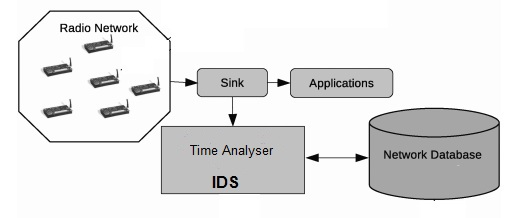
\includegraphics[width=0.5\textwidth]{IDS_fw}	
    \caption{IDS Framework}
    \label{fig:ids_fw}
\end{figure}
The IDS framework components has been shown in \ref{fig:ids_fw}.
The IDS has three kinds of components --- 
\begin{inparaenum}
\item the motes in the WSN that are subject to legitimate or illegitimate update; 
\item an IDS transport client (ITC) application that runs on the sink and works in coordination with the IDS to assists in intrusion detection; and
%The sink is protected from all kinds of security breaches whether it is physical or logical. 
\item an IDS application that runs on a system with higher computing resources which is physically attached to the sink, and houses a network database (NDB).
\end{inparaenum}
These components works in a unified fashion to make the IDS work.

The chronology of the activities that take place in a WSN in a software  update and are associated with the IDS shown in \ref{fig:ids_fw}.
\begin{inparaenum}
\item Updates are initiated using deluge protocol;
\item Deluge disseminates the new software image using the motes enroute to reach all the motes using a relay mechanism; 
\item The nodes deliver their timing information to the sink using an AM packet;
\item AM packets from the distant nodes rely on the other nodes enroute to reach the sink using a relay mechanism; and
\item The ITC application in the sink delivers revelent information to the IDS for processing. 
\end{inparaenum}
The IDS analyses the acquired timing information to arrive at decision.
\begin{figure}[btp]
    \centering
    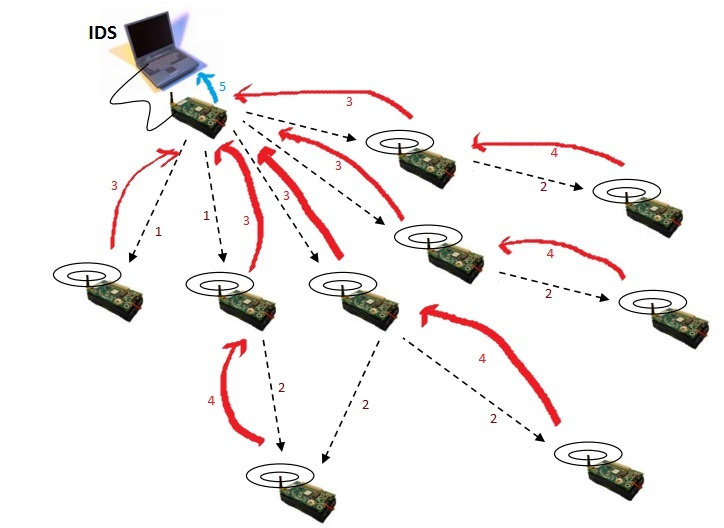
\includegraphics[width=0.5\textwidth]{IDS}
	%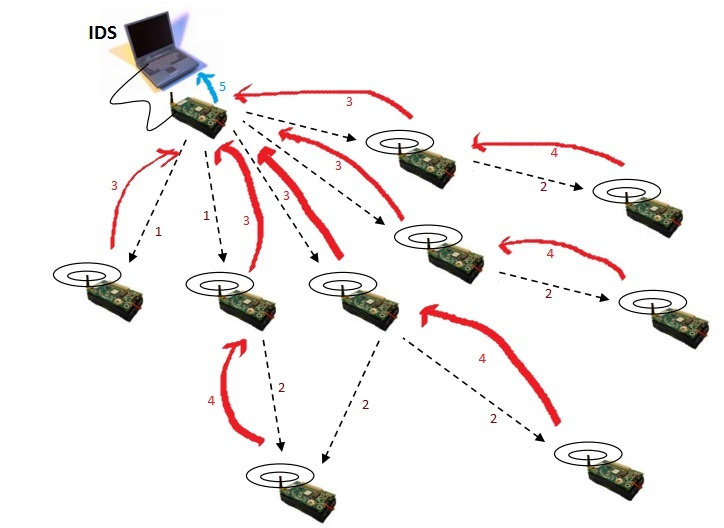
\includegraphics[scale=0.5, angle=180]{IDS}
    \caption{IDS Modelling}
    \label{fig:ids_model}
\end{figure}

\subsubsection{Determining IWS}
\label{ssc:cal_iws}

The intrusion detection activity begins with the action of motes in the network by endorsing update time. 
Once updated with new software image, each node initiates an AM with the update time information to the sink. 
An AM packet initiated for the IDS has several fields: destination address, type identifier that indicates the update time information and the protocol for IDS, timing information and a checksum value.
%[DO WE WANT TO INCLUDE THE PATH TAGGING; MAY BE LATER - IT INCREASES RELIABILITY, NOT DIRECTLY $IDS$ ACTIVITY?]
%[path tagging is good, but in all cases, what’s the risk from intruders messing with the reported data?]
%[PATH TAGGING CAN BE USED AS HEART-BEAT MESSAGE]
The packet travels through the network using existing transport layer protocols.
When it arrives at the sink, the checksum value is examined by the ITC to ensure that the packet content has not been altered enroute.
The ITC then inserts the update time, mote ID and related information to the NDB in the IDS.
The IDS maintains an identifier to differentiate among different update times from different runs for the same mote.

The first software update run in the WSN is considered to be legitimate and the IDS takes this timing information as baseline.
It is possible and desirable that the IDS is trained with several other update runs.
More training improved the ability of the IDS to detect intrusion more accurately.
Utilising multiple runs are useful and beneficial as it increases accuracy and dependency.
However, the IDS needs to be manually controlled to enable multiple training runs.
Outcome from these runs are statistically treated to build the baseline.


Once the IDS baseline has been built, all subsequent updates are liable to scrutiny by the IDS.
The timing analyser module in the IDS inspects the NDB once an update activity has been detected.
It determines the changes in the statistics of the update time and calculates IWS based on following utility function:

\begin{equation}
\label{eqn2} 
	\mathit{IWS} = \sum \limits_{i=0}^{n} \frac{\left| \mu_i - t_i \right|}{\sigma_i + 1}
%	f_1 = \sum\limits_{i=0}^{n} \left( \mu_i - t_i \right)
	\end{equation}
where, 

	\hspace {.2cm} $i$ --- Identification of the Mote  
	
	\hspace {.2cm} $t_i$ --- Image Update Time at Mote \emph{i} 
	
	\hspace {.2cm} $\mu_i$ --- Mean Update Time at Mote \emph{i} 
	
	\hspace {.2cm} $\sigma_i$ --- Standard Deviation of Update Time at Mote \emph{i} 
	

\subsubsection{Building Intrusion Warning Zones}
\label{ssc:iw_zone}

Threshold for building of Intrusion Warning Zone (IWZ) depends on the assumed ability of the IDS having IWS knowledge of all possible intrusions in the network.
Such knowledge can be built by replicating intrusion activity from all nodes in the network once.
However, in case where it is not possible, replicating intrusion activity from the furthest few nodes may serve the purpose.
IDS can build a scale of possible expected range of IWS for the deployed topology and can classify the IWS in different zones to imply certain warning level.

The IDS considers an IWS upto 10\% from the scale to be safe and marks as `GREEN' zone, an IWS above 30\% to be possible intrusion and is marked as `RED' zone.
However, an IWS within the range of 10\% --- 30\% can neither be considered safe, nor an intrusion, hence is marked as `GREY' that indicates a situation where rules are not known.
However, the thresholds are not conclusive and may require some variation based on the density, power level used in the WSN and scale of deployment.

\subsubsection{Database Structure}
\label{ssc:db}
The NDB stores the statistics of the update time of all the motes in the WSN for each update applied.
It consists of three flat tables that performs as storage.
The tables have been  designed to improve the IDS performance. 
First, In-Network Activity Table (INT) consists of the  following fields:
\begin{verbatim}
mote_id, timestamp, id_seq, 
upd_seq, upd_type, zone_type
\end{verbatim}
where, $mote\_id$ is the source node ID, $timestamp$ is the time when the new software image starts executing, $id_seq$ is the number of times an update arrived from same $mote\_id$, $upd\_seq$ is the number of time an update has been initiated from the sink.
The unique key for INT is $mote\_id$, $upd\_seq$ pair.
$upd\_type$ indicates if the record belonged to a baseline update.
For a baseline update type, the $zone_type$ is $zero$, while for others it is updated to indicate if the update related to that particular mote from that particular run was processed as GREEN, GREY or RED.

Secondly, the Baseline Table (BLT) holds the processed information from the legitimate runs and has the following fields:
\begin{verbatim}
mote_id, mu, sigma
\end{verbatim}
where, $mote\_id$ is the source node ID, $mu$ is the mean time and $sigma$ is the standard deviation for each $mote\_id$ from all legitimate runs.

Finally, the Intrusion Activity Table (IAT) filters out necessary information from INT about most recent software update and contributes to the performance of the IDS.
The table has two fields:
\begin{verbatim}
mote_id, timestamp
\end{verbatim}
where, $mote\_id$  and $timestamp$ are same as the corresponding fields in INT.
Every time a decision on an update has been made and a new update is detected, this table is flashed.

\subsubsection{Activities in the Network}
\label{ssc:actnet}
As part of enhancement into the deluge protocol, the motes are enriched with the prior knowledge of the sink or sinks in the WSN.
Whenever an update takes place in a mote, it reboots with the new software running and stores the bootup time in its memory.
I NEED TO CONFIRM IF THE TIME IS ALREADY SAVED WITH THE IMAGE AS PART OF DELUGE PROTOCOL IMAGE/GOLDEN IMAGE.
The locally stored information  is used later in case it requires to recover from packet delivery failure.
The information $type$, $mote\_id$,  $time\_stamp$,$upd\_seq$ are packed along with an additional checksum in an AM packet and forwarded to the sink/sinks.
The AM has the following information in the packet:
\begin{verbatim}
|------------------------------------------|
|Source|-----------------------------------|
|  ID  |msgtype|timestamp|upd_seq|checksum||
|------|-----------------------------------|

Figure: Need to draw a better picture
\end{verbatim}
The AM packet is relayed through the network to the sink.

\subsubsection{Activities in the Sink}
\label{ssc:actsink}
As an AM arrives from the radio network to the sink, the ITC application running on the sink verifies the checksum.
If the checksum fails, the packet is discarded and failure recovery is initiated once only in coordination with the IDS.
However, if the AM passes checksum, the ITC application extracts the relevant information and populates the INT in the resident host system. 

\subsubsection{Activities in the IDS}
\label{ssc:actids}
An update is typically initiated from the host system where the IDS resided.
The IDS constantly monitors the programming port and coordinates with the ITC. 
They automatically identify the first update as input for baseline training data.
It is possible to put the IDS in training mood for extended number of updates.
Result from all updates run during the training period are statistically treated to build the baseline.
Though the IDS can work theoretically with a single update, it is recommended to have minimum three updates for the training phase while running more training updates is desirable.
For our experiments, we have considered 20 runs for each topology.

Once the training phase ends, the IDS calculates mean and standard deviations at each of the motes and stores the  information on BLT.
It also stores the number of update runs it considered for the BLT.
This number contributes two folds:
\begin{inparaenum}
\item it indicates the reliability of the training data / baseline; and
\item the number is used for statistical processing in case there is a need to increase the training data at a later time or data from an update is identified as acceptable is automatically included in baseline computation and the BLT is updated.
\end{inparaenum}
Once the BLT has been built, the IDS runs on active mood and all updates are subject to intrusion checks.
When an update is initiated in the WSN, data pushed into the INT are filtered and relevant information related to the ongoing update populates the  IAT.
The IDS waits upto a specific time, which is determined by the maximum time taken to complete a network-wide  update during the training phase, before it reports the findings about intrusion possibility.
While the procedure described above is quite straight forward, it gets complicated because of the unreliable packet transmission pattern experienced by WSN due to node failure, link failure and node reboot \cite{aro04}, \cite{bec04}.
IDS reports the findings with a provision of updating it later when an expected data from certain mote are not available within reasonable time.
In such case, the IDS employs a packet recovery mechanism to obtain necessary information.

The packet recovery mechanism is initiated when a valid packet is not available form one or more motes within  the  determined maximum time from the updates  during the training phase.
Upon receiving signal from the IDS, the ITC initiates AM to the specific requesting a retransmission of the update time and waits further  triple time for the required AM packet. If the packet is available,  IWS is recomputed and decision is updated accordingly.
If the packet is still not available within specified time, the node is marked as compromised or failed and a notification is generated.



%They exhibit highly transient loss patterns that are susceptible to changes in environmental conditions [21]. Asymmetric links are common, and prior work has shown network behavior to often be worse indoors than out, predominantly due to multi-path effects [22]. 
%Y. Sasson, D. Cavin, and A. Schiper. Probabilistic broadcast for flooding in wireless networks. Technical Report IC/2002/54, 2002.
%22 R. Szewczyk, J. Polastre, A. Mainwaring, and D. Culler. Lessons from a sensor network expedition. In Proceedings of the 1st European Workshop on Wireless Sensor Networks (EWSN '04), January 2004.



%PacketLink is most reliable when software acknowledgements are enabled   as opposed to hardware auto acknowledgements.
%    
%What is the new idea I wanted to introduce?
%What are the threats we want to deal and why?
%Why do we limit our scope here; why detect and not prevent?
%
%%What is our hypothesis about the solution?
%Network based intrusion detection attempts to identify unauthorized, illicit, and anomalous behavior based solely on network traffic. A network IDS, using either a network tap, span port, or hub collects packets that traverse a given network. Using the captured data, the IDS system processes and flags any suspicious traffic. Unlike an intrusion prevention system, an intrusion detection system does not actively block network traffic. The role of a network IDS is passive, only gathering, identifying, logging and alerting
%How in theory we want to solve it?
%
%How did we conduct our experiment?
%Details of methodologies.
%
%What are the topologies we have tested? 
%What are the rationale for choosing these topologies?
%What are the results we found?

%This section makes the experiment reproducible
%How did we do what we wanted to find out
%This is what we did in order to answer the question
%
%\section{Results}
%What did you find out and nothing more
%Following hypothesis were tested
%For hypothesis -1, this was found 
%and then others hypothesis results
%




\section{Evaluation}
\label{sec:eval}

%the results they achieved using those methods. In addition, they present their analysis of the data and describe some of the interpretations and implications of their work.
%The data collected during the research are presented in this section, both in written form and using tables, graphs, and figures (see our Using Graphs and Visual Data module). In addition, all statistical and data analysis techniques used are presented (see our Statistics in Science module). Importantly, the data should be presented separately from any interpretation by the authors. This separation of data from interpretation serves two purposes: First, it gives other scientists the opportunity to evaluate the quality of the actual data, and second, it allows others to develop their own interpretations of the findings based on their background knowledge and experience. 
%include both the raw data and their analysis. Keeping the raw data (in the form of a photograph) facilitated reanalysis by other scientists:

%Discussion and conclusions: In this section, authors present their interpretation of the data, often including a model or idea they feel best explains their results. They also present the strengths and significance of their work. Naturally, this is the most subjective section of a scientific research article as it presents interpretation as opposed to strictly methods and data, but it is not speculation by the authors. Instead, this is where the authors combine their experience, background knowledge, and creativity to explain the data and use the data as evidence in their interpretation 
% Often, the discussion section includes several possible explanations or interpretations of the data; the authors may then describe why they support one particular interpretation over the others. This is not just a process of hedging their bets – this how scientists say to their peers that they have done their homework and that there is more than one possible explanation. In the woodpecker article, for example, the authors go to great lengths to describe why they believe the bird they saw is an ivory-billed woodpecker rather than a variant of the more common pileated woodpecker, knowing that this is a likely potential rebuttal to their initial findings. A final component of the conclusions involves placing the current work back into a larger context by discussing the implications of the work. The authors of the woodpecker article do so by discussing the nature of the woodpecker habitat and how it might be better preserved.

\begin{table*}[t!]
\centering
\begin{tabular}{|l|*{20}{r|}r}
\hline
\bd{Node ID}           & \bd{1} & \bd{2} & \bd{3} & \bd{4} & \bd{5} & \bd{6} & \bd{7} & \bd{8} & \bd{9} & \bd{10} & \bd{11} & \bd{12} & \bd{13} & \bd{14} & \bd{15} & \bd{16} & \bd{17} & \bd{18} & \bd{19} & \bd{20} \\
%Mote ID           & 1 & 2 & 3 & 4 & 5  & 6 & 7 & 8 & 9 & 10 & 11 & 12 & 13 & 14 & 15  & 16 & 17 & 18 & 19 & 20 \\
\hline

$\mu$            & 0 &19 & 19& 69&139 &213&276&344&377&432 &432 &432 &377 &335 &273 & 207&137 & 68 & 17 & 19 \\
$\sigma$		 & 0 & 5 & 5 & 6 & 22 & 36& 37&43 &44 & 44 & 44 & 44 & 44 & 45 & 44  & 33 & 24 & 5 & 3 & 5 \\
$\mathit{IWS}$
                 &0.01&16 &19 &73 & 140 &203 &246 &336 &344 &396 &395 &535 &406 &332 &269 &237 &113 & 72& 16 & 16 \\

%                 &\green{0.01& 16 & 19} &\grey{73 & 140} &\red{203 & 246 & 336 & 344 & 396 & 395 & 535 & 406 & 332 & 269 & 237} &\grey{113 & 72}& \green{16 & 16} \\
\hline
\end{tabular}
\caption{Mean and Standard Deviation of motes and IWS from intrusion at motes. Further explained in Figure-\ref{fig:ellip}}
\label{tab:ellip}
\end{table*}


\begin{figure*}[t!]
\label{fig:ellip}
    \centering
    \begin{subfigure}[b]{0.5\textwidth}
        \centering
        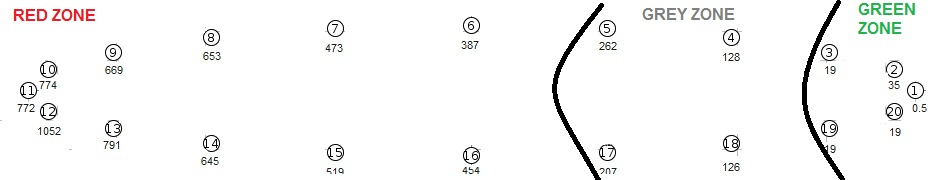
\includegraphics[height=1in, width=4in]{Elliptical}
        \label{subfig:elliptopo}
        \caption{IWS and Relative position of nodes}
    \end{subfigure}%
    ~ 
    \begin{subfigure}[b]{0.5\textwidth}
        \centering
        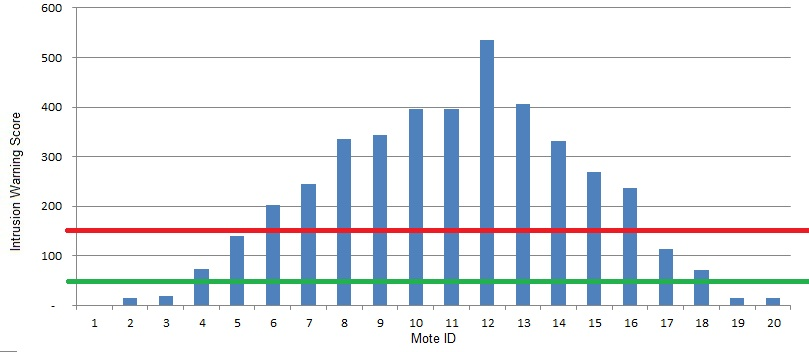
\includegraphics[height=1.2in]{Elliptical_column}
        \label{subfig:ellipgraph}
        \caption{Comparison of IWS at different motes}
    \end{subfigure}
    \caption{Relative position and comparison of IWS for intrusion at different motes from data in Table-\ref{tab:ellip}}
\end{figure*}


The performance and effects of the proposed IDS were tested in different topologies, such as linear, circular, elliptical, double rings, wide lines/grid, tree, and other topologies.
While discussing all of these topologies are useful, we shall concentrate our discussion on results and findings elliptical topology only.
Diiscussing any of the topologies presents fair idea about the outcomes from the others. 
We shall mention the cases when the outcome was considered to be exception and contrary to the expectations.
The space requirement also motivates us to limit the discussion to necessary details only.


%\subsection{Data1 + Discussion}

We have selected data from elliptical topology for several reasons.
Ellipse has a shape which is almost midway among the range of topologies between a circular and a linear one.
Extending the minor axis of the ellipse makes the topology equivalent to a circle, while contracting it is equivalent to a grid or even a linear topology.
Thickening the perimeter of the circle turns it into a double ring.
Again, the linear topology can be considered as a tree with one or two branches.
Extending it with more branches presents a fairly complex tree structure.
Because of these similarities, discussing elliptical topology is an interesting choice.


The shape of the ellipse has been designed considering several requirements.
The ellipse shape deployment has been shown in Figure-\ref{subfig:elliptopo}.
The motes on either side of minor axis remained within each others transmission range, whereas motes on the either side of the major axis did not.
Total 20 nodes were deployed with the minor axis being 30 meter and the major axis being way larger than that.
The transmission power level was set at 100\% which allowed a  transmission range of 50 meter and nodes were  able to interfere other nodes at  upto 100 meter apart.
The motes were placed at a space of 35 meter along the circumference of the ellipse. 
The deployment enabled multiple transmission paths to all the motes.
It contributed to achieve  redundancy and  reliable image transfer. 

The simulations proceeded without interruption and produced expected results.
To build the baseline data, we assigned mote ID 1 as the sink and ran 20 updates initiated from the sink.
The output from these runs were processed as describes in Section-\ref{ssc:build_baseline} and were statistically treated to compute the `mean' and `standard deviation' of the  time at which each of the nodes were updated with the new image.
The computation results have been presented in Table-\ref{tab:ellip}.

Once the baseline data were built, intrusion scenarios were replicated at other nodes according to the experiment protocols.
Output of these replications were processed to compute IWS.
Results obtained from these simulated intrusions are also reported in Table-\ref{tab:ellip}.

IWS shown in the last row of Table-\ref{tab:ellip} were used to build a scale that ranged from $0$ to maximum of $\mathit{IWS}$.
Building this scale was crucial for the ability to classify the IWS to meaningful zones.
However, it is not possible to build the scale without the knowledge of the expected IWS from the furthest nodes in the network.
Nevertheless, we established two threshold levels at 10\% and at 30\% that were useful in zone classification using intuitive heuristics.
Details of the zoning has been discussed in Section-\ref{ssc:iw_zone}.


Table-\ref{tab:ellip} shows the statistical measurements obtained at different motes and the IWS measured when each of the motes were considered as intrusion point.
It can be clearly seen that IWS at the intrusion points differ considerably.
The first row in Table-\ref{tab:ellip} contain the Node IDs that are headers for the data displayed underneath.
The next two rows describe the `mean' and `standard deviation' that were computed from the 20 legitimate updates initiated from the sink.
Cells in the last row contain the IWS calculated using  the utility function shown in Equation-\ref{eqn2} for the test runs initiated from the node indicated at top of the column.
The data shown in the table can best be interpreted when related to Figure-\ref{fig:ellip}. 
Figure-\ref{subfig:elliptopo} shows the actual relative positions of the motes with mote ID written at the center of the tiny circle and IWS measured when an intrusion attempt has been initiated from the mote. 
The figure additionally divides the region in GREEN, GREY and RED zones according to the logic discussed in \ref{ssc:actids}.
The graph in  Figure-\ref{subfig:ellipgraph} shows the relative measures of the IWS from the motes.

From the data presented in Table-\ref{tab:ellip}, analysing the baseline data we find that the motes further away from the sink are found to have higher `mean' and `standard deviation' in terms of update time.  
However, `standard deviation' raises gradually, though it does not vary to a great extent for relatively small distance difference when multiple paths are present.
This results from the  availability of more redundant paths make the image transfer more efficient and reliable which contribute to the stability of `standard deviation'.
Therefore, even remaining at considerably different distances from the sink, mote ID 8, 9, 10, 11, 12, 13, 14 and 15  have quite similar `standard deviation' of update time.
In contrast to this, `mean' increases sharply as the motes are placed further from the sink.
The quantities established from the baseline data shows that motes closer to the sink have lower `mean' which increases sharply with the increase in distance.


The utility function presented in Equation-\ref{eqn2} is designed to neutralise the undesired %/unexpected
changes in `mean' and `standard deviation' which are expected to contribute to a near $zero$ IWS.
A near $zero$ IWS is further classified as GREEN zone to indicate a legitimate software update. 
Table-\ref{tab:ellip} and Figure-\ref{fig:ellip} shows defined zones and IWS measured when intrusion was initiated at different motes.

The IWS increases linearly with the increase in distance from the sink.
The `distance' term can be misleading in the context of our discussion and demands further clarification.
Euclidean distance between a mote and the sink does not make useful sense as the packets in the network must travel using a relay mechanism through other motes in the network.
Because of the availability of the multiple paths, it is not possible to quantify the exact distance that a packet would travel while transporting form a mote to the sink.
However, an estimation of distance along the most probable link path based on the connectivity may be considered.

IWS is considerably higher for intrusion at distant motes than ones which are close to the sink.
This phenomena is topology dependent, which also implies   that it is connectivity dependent.
It is possible that if IWS in a network are organised in a specific order, it would represent/resemble   the original topology in some fashion.
For example, in the elliptical topology, the link path between node 1 and node 11 through node 5 is represented by a curve with a positive slope or rise.
On the other hand, the link path through node 15 is represented by a fall or a negative sloped curve.
There is a relationship between the curvature/eccentricity of the original topology and the represented curve or  trend.
%This implication would be more evident once we discuss more topologies in the upcoming paragraphs. {Only if we discuss the other topologies}.
However, establishing the relationship is beyond the scope of this paper.

%\subsection{discussion of contributions}


\begin{table*}[t!]
\centering
\begin{tabular}{|l|*{20}{r|}r}
\hline
\bd{Node ID}           & \bd{1} & \bd{2} & \bd{3} & \bd{4} & \bd{5} & \bd{6} & \bd{7} & \bd{8} & \bd{9} & \bd{10} & \bd{11} & \bd{...} & \bd{31} & \bd{32} & \bd{33} & \bd{34} & \bd{35} & \bd{36} & \bd{37} & \bd{38} \\
%Mote ID           & 1 & 2 & 3 & 4 & 5  & 6 & 7 & 8 & 9 & 10 & 11 & ...& 31 & 32 & 33  & 34 & 35 & 36 & 37 & 38 \\
\hline		\hline

Power	  &  &  &  &  &  &  &  &  &  &  &  &  &  &  &   &  &  &  &  &  \\
$100\% $          & 512 & 529 & 512 & 512 & 512  & 512 & 476 & 478 & 476 & 459 & 458 & ...& 49 & 47 & 53  & 48 & 49 & 51 & 47 & 29 \\
\hline

Power	  &  &  &  &  &  &  &  &  &  &  &  &  &  &  &   &  &  &  &  &  \\
$50\%$            &31 & 59&254& 31& 31 &283& 32& 32& 254& 31 &253 & ...& 31 & 31 & 31  & 30 & 31 & 31 & 30 & 0 \\
\hline
\end{tabular}
\caption{IWS from intrusion at motes in `Owheo Sensor Network'. Further explained in Figure-\ref{fig:owheo}}
\label{tab:owheo}
\end{table*}


\begin{figure*}[t!]
\label{fig:owheo}
    \centering
    \begin{subfigure}[b]{0.5\textwidth}
        \centering
        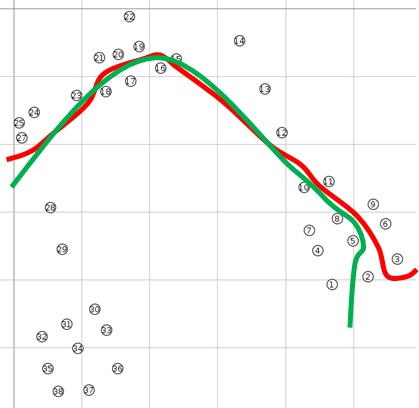
\includegraphics[height=2.5in]{Owheo_full}
        \label{subfig:owheo_full}
        \caption{Zone boundary at Full Power Level}
    \end{subfigure}%
    ~ 
    \begin{subfigure}[b]{0.5\textwidth}
        \centering
        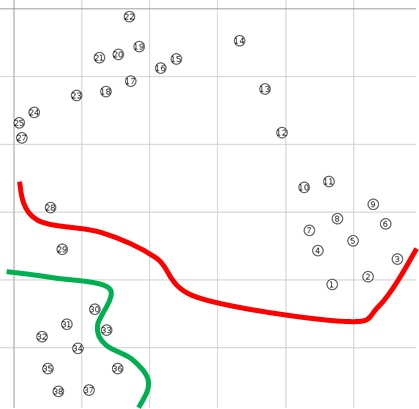
\includegraphics[height=2.5in]{Owheo_half}
        \label{subfig:owheo_half}
        \caption{Zone boundary at Half Power Level}
    \end{subfigure}
    \caption{Comparison of Zone boundary for power level variations in `Owheo Sensor Network'. IWS of the motes at the power levels are shown in Table-\ref{tab:owheo}}
\end{figure*}

The main contribution of this research project comes from the fact that the IDS is able to report an anomaly from a software update in quantitative term like the IWS.
The claim is evident from the data presented in Table-\ref{tab:ellip}.
For example: in this case, a regular legitimate update would be initiated from node ID 1. 
When such a scenario was simulated and the timing information was compared against the baseline, it resulted into a IWS of 0.01.
The result matched the theoretical expectation, as a legitimate update initiated from the sink should produce a near $zero$ IWS.
On the other hand, when intrusion scenario were simulated from the nodes near the sink, the IWS reported was fairly low, e.g. 16 for mote ID 2, 19, and 20
 and 19 for node 3 
 and likewise.
Because of the fact that IWS of the motes close to the sink are likely to be very low, which is in line with the theoretical expectation, it is quite difficult to conclude if such a IWS indicate an intrusion. 
However, for the distant motes, the IWS is quite high and the IDS can easily conclude as intrusion, e.g. IWS of 246 for mote ID 7, 269 for mote ID 15, 395 for mote ID 11, 535 for mote ID 12 and likewise indicate intrusion.


While reporting severity or likelihood of an intrusion in quantitative term like the IWS is useful, it is more beneficial if the quantity is associated with some kind of interpretation.
The technique of associating such interpretation has been discussed in Section-\ref{ssc:iw_zone} and in this Section. 
In the elliptical topology intrusion scenario, maximum IWS reported in the presented data in Table-\ref{tab:ellip} was 535. 
Motes reporting an IWS upto 53.5 would be considered in the GREEN zone.
For example, in figure-\ref{subfig:elliptopo}, mote ID 2, 3, 19, and 20 are in this zone.
On the other hand, IWS above 53.5 and bellow 160.5 are considered to be in the GREY zone. 
Motes in this zone are 4, 5, 17, and 18.
They can neither be considered free from intrusion, nor it is possible to easily arrive at a decision that the scores indicate intrusion for sure.
In contrast to both the scenario describes above, IWS above 160.5 is considered to be an intrusion.
All other motes in the topology have a IWS above this threshold level and hence are considered to be more susceptible to intrusion.

The idea of zoning associated with the IWS is very beneficial in securing a WSN.
It is immensely useful in designing a secure network deployment, which is considered to be another major contribution of the research work.
The motes which are found to be in the GREEN zone must be adequately secured by design with additional physical security as intrusion in these motes are not observed by the IDS.
On the other hand, motes in the GREY zone need additional monitoring which would aid determining if the IWS indicated a real intrusion or a false positive.
The additional monitoring could be in the form of an algorithmic or physical observation or listening post or even employing additional protocol.
The rest of the region, identified by the RED zone, is under the effective surveillance of the IDS and is considered to be secure.

The concept of zoning using the IDS is a very useful tool in designing secure WSN deployment.
A network is more secure when it has a smaller GREEN and GREY zone.
A smaller GREEN zone implies the requirement of lesser resources to impenetrably secure less number of motes.
Similarly, a smaller or non-existent GREY zone would lesser monitoring measures.
Such a secure WSN can be designed by physically relocating some of the motes or even by varying the factors like power level.
For example, we have simulated the IWS scenario of the `Owheo Sensor Network' at two different power levels in our quest to design a secure WSN using the IDS.
`Owheo Sensor Network', which is the WSN deployed in the Department of Computer Science building at the University of Otago, is intended to be used for research purposes.




Table-\ref{tab:owheo} shows the IWS at different motes as intrusion points at 100\% and 50\% power levels. 
In `Owheo Sensor Network', mote ID 38 was marked as the sink and mote ID 26 does not exist.
At 100\% power level, 19 nodes (mote ID 1, 4, 5, 7, 8, 10, 16, 17, 18, 28, 29, 30, 31, 32, 33, 34, 35, 36, and 37) were in GREEN zone, only one node (mote ID 2) was in GREY zone and the rest 16 nodes were in RED zone.
The deployment and the zoning boundaries at 100\% power level has been shown in Figure-\ref{subfig:owheo_full}.
When the same deployment was simulated at 50\% power level, only seven nodes (mote ID 30, 31, 32, 34, 35, 36, and 37) were in GREEN zone, two nodes (mote ID 29, and 33) were in GREY zone and rest 27 motes were in RED zone.
The deployment and the zoning boundaries at 50\% power level has been shown in Figure-\ref{subfig:owheo_half}.
Comparing the scenarios presented in  Figure \ref{subfig:owheo_full} and \ref{subfig:owheo_half}, it can clearly be established that Figure-\ref{subfig:owheo_half}, i.e. deployment at 50\% power level is more secure than the other because of two reasons:
\begin{inparaenum}
\item it has a smaller sized GREEN and GREY zone; and 
\item there are lesser number of nodes in these zones. 
\end{inparaenum}
The deployment can be made more secure by physically relocating some of the motes from GREEN zone to RED zone, provided the relocation does not hamper the original intended purpose of the WSN.



%Identifying node failure and node compromise
The IWS is also able to detect node failures in the WSN.
This additional advantage comes as a by-product contribution.
However, as this was not a design consideration, the contribution is robust enough, yet it is worth mentioning.
The case of a node not reporting its update time within a specified delay is handled by a error recovery procedure put in place by the IDS.
If the recovery procedure described in section-\ref{ssc:actsink} fails, there is a possibility that the node might have failed or have been compromised.
However, such failure resulting into contributing towards an IWS which is quite different for the update pattern detected from the timing information reported by the other nodes.
The IDS structure is such that it has an expected pattern and shape of IWS for an intrusion at some specific point.
If the shape is distorted to a great extent, it indicates some unusualness which can be attributed to some other phenomena like node failure or compromise.
The node failure or node compromise can take place concurrently with or without intrusion.
It might also indicate a different type of attack associated with a physical intrusion.
An interpretation form the IDS view of the topology would enable identification of some other types of attacks in WSN like node relocation, node repudiation, node compromise.




%\subsection{Discuss other topologies}

%Not included in this paper. Already long enough.
%Insight for secure deployment. which topologies would work better - idea
%Insight for a deployment that would ensure better connectivity
%
%
%Interpretation of the results.
%Our argument in support of the results.
%
%Explanation of the results to answer the question - so what.
%Why the result was important.
%Why does this matter .

%Constraints and limitations of the program
%Opportunities for future work

% Must explicitly state what is my contribution
% If there are some recommendations, must include them here
%What are my specific contributions to the academic society?
%Do I have some recommendations about it?


\section{Conclusion}
\label{sec:conc}
Building secure WSN is of paramount importance, yet it is quite difficult.


Wrap the whole thing up;
\subsection{write here}
%%%%OWN Notes

%state-of-the-art methodologies in IoT security, implementation, applications, modeling for threats detections and countermeasures; 
%illustrate the benefits of detection and prevention threats applications in IoT networks, modeling, and analysis. 
%Identify the main issues that face efficient and effective countermeasures implementation in IoT security; 
%demonstrate by examples how the performance of IoT security can be evaluated. 
% cutting-edge research on threat detections, preventions, and countermeasures of IoT security; 
%present the trends in countermeasures (modeling, application, analysis, etc); 
%discuss the main features of current IoT security simulations. 
%Point out the main trends in IoT security evaluation and their tools, 
%IoT simulators, 
%Compilation of the problems that arise during the use of IoT security and the solutions that are applied to them. 

%Who are benefitted from the research outcome
%=============== ===============
%academics, researchers, post-graduate students, developers, professionals, network designers, network analysts, telecommunication system designers, technology specialists, practitioners, computer network security professionals. 
% researchers and academicians who identify methodologies, concepts, tools, and applications through reference citations, literature reviews, quantitative/qualitative results, and discussions.
% reference at university libraries, academic institutions, research and development centers, information technology centers, and any institutions interested in using, designing, modeling, and analyzing computer networks security
% text  for courses teaching computer networks security, simulation, and modeling for under/post graduate students. 

%Recommended Topics 
%==================================== 
%Definition, features and types of IoT. 
%Implementation, application and modeling for threats detections and countermeasures destined for IoT networks. 
%State-of-the-art methodologies in IoT security. 
%~ IoT and privacy. 
%~ IoT and Integrity. 
%~ IoT and Confidentiality. 
%~ IoT and Authentication. 
%~ IoT case studies, field studies, and applications. 
%~ IoT implementation issues. 
%~ User experience with IoT. 
%~ User interface of IoT technology. 
%~ Demonstrate by examples how the performance of IoT security can be evaluated and measured. 
%~ Introduce the most popular academic and professional IoT simulators in which security can be implemented. This includes discussion on the main features of current IoT security simulations. Also it includes demonstration by examples how the performance of IoT security can be evaluated and measured. 

%http://www.wikicfp.com/cfp/servlet/event.showcfp?eventid=38207

Signature\hspace{0.5cm} \makebox[1.5in]{\hrulefill}
\begin{tabbing}
Contact Address: \= 128, Owheo Building\\
\> 133, Union Street (West)\\
\> Dunedin - 9010, New Zealand
\end{tabbing}



\bibliographystyle{IEEEtran}
\bibliography{bare_conf}

\end{document}


